\chapter{Background Research}\label{ch:Background}

This chapter provides the theoretical foundation and literature context for the forecasting methods used in this project. It begins with an overview of electricity demand forecasting, examines the influence of weather variables, reviews classical and machine-learning approaches, and then presents in-depth descriptions of the two core techniques---CatBoost and Phasor Particle Swarm Optimisation (PPSO)---that form the proposed hybrid model.


\section{Electricity Demand Forecasting: An Overview}

Electricity demand forecasting is the process of estimating future electricity consumption based on historical data, weather conditions, and other contextual variables. Forecasts are categorised by their prediction horizon \parencite{amasyali2018review}:

\begin{itemize}
    \item \textbf{Very short-term} (minutes to a few hours): used for real-time grid balancing.
    \item \textbf{Short-term} (one day to one week): used for generation scheduling and fuel procurement.
    \item \textbf{Medium-term} (one month to one year): used for maintenance planning and contract negotiation.
    \item \textbf{Long-term} (one year and beyond): used for infrastructure investment and policy formulation.
\end{itemize}

This project focuses on \emph{short-term daily} forecasting, where the objective is to predict the total electricity demand (in MWh) for the next day. Short-term forecasts are critical because they directly influence operational decisions such as unit commitment, spinning reserve allocation, and spot-market trading strategies \parencite{akay2007grey}.


\section{Role of Weather Variables in Electricity Demand}

Weather conditions are among the most significant external drivers of electricity consumption, particularly in climate-sensitive regions. The key weather variables and their effects on demand are summarised below.

\subsection{Temperature}

Temperature has the most direct and well-documented impact on electricity consumption. In tropical climates such as Singapore, higher ambient temperatures increase air-conditioning load, which constitutes a substantial portion of total electricity demand. The relationship between temperature and demand is non-linear: moderate temperature variations produce limited changes in consumption, whereas extreme heat triggers sharp demand spikes as cooling systems operate at full capacity \parencite{zhao2012review}. In this project, the daily mean air temperature at 2\,m height is used as the primary weather predictor.

\subsection{Humidity}

Relative humidity amplifies the perceived thermal discomfort beyond what temperature alone indicates. High humidity reduces the effectiveness of evaporative cooling, prompting occupants to increase air-conditioning usage even when air temperatures are moderate. The interaction between temperature and humidity is captured in this project through a \emph{Comfort Climate Index} (CCI), defined as:
\begin{equation}\label{eq:cci}
    \text{CCI} = T + 0.55 \times (1 - \text{RH}/100) \times (T - 14.5)
\end{equation}
where $T$ is the mean daily temperature ($^\circ$C) and RH is the mean daily relative humidity (\%). The CCI provides a single metric that approximates the combined thermal stress experienced by building occupants.

\subsection{Solar Radiation and Wind Speed}

Daily cumulative shortwave radiation ($\text{W/m}^2$) affects demand through its correlation with daytime temperatures and, in buildings with significant glazing, through direct solar heat gain. Wind speed influences the rate of convective heat exchange and may reduce or increase cooling demand depending on the prevailing conditions. Both variables are included in the feature set as secondary weather predictors.

\subsection{The Singapore Context}

Singapore's equatorial location (1.35$^\circ$N, 103.82$^\circ$E) produces a consistently warm and humid climate with minimal seasonal temperature variation. However, the monsoon seasons---Northeast Monsoon (December--March) and Southwest Monsoon (June--September)---introduce variability in rainfall, cloud cover, and humidity patterns that can influence daily demand. Unlike temperate regions where heating load creates a U-shaped temperature--demand relationship, Singapore's demand is monotonically increasing with temperature, simplifying the modelling task but also reducing the signal-to-noise ratio for marginal temperature changes.


\section{Classical Forecasting Methods}

\subsection{ARIMA and Exponential Smoothing}

Autoregressive Integrated Moving Average (ARIMA) models capture linear temporal dependencies by modelling the relationship between past observations and future values. These models require the time series to be stationary (or transformed to achieve stationarity) and are effective when demand follows regular, repetitive patterns. Exponential smoothing methods (e.g.\ Holt-Winters) assign greater weight to recent observations, allowing adaptation to trends and seasonality \parencite{almusaylh2018forecasting}.

However, both approaches assume linear relationships and cannot easily incorporate exogenous variables such as weather without extensions (e.g.\ SARIMAX). Their inability to model non-linear interactions limits their accuracy in complex multi-variable forecasting scenarios.

\subsection{Regression-Based Methods}

Linear and polynomial regression models extend classical forecasting by incorporating external predictors. These methods are interpretable and computationally inexpensive but struggle with the non-linear, threshold-dependent relationships between weather variables and electricity demand. As Schirmer et al.\ \parencite{schirmer2019evaluation} demonstrated, linear regression is consistently outperformed by tree-based methods in residential energy consumption prediction tasks.


\section{Machine Learning for Demand Forecasting}\label{sec:ml_forecasting}

Machine learning methods learn patterns directly from data without requiring explicit assumptions about functional form. The following subsections describe the specific algorithms used in this project.

\subsection{Random Forest}

Random Forest \parencite{breiman2001randomforest} is an ensemble method that constructs multiple decision trees during training and outputs the mean prediction of the individual trees. Each tree is trained on a bootstrapped sample of the data, and at each split, a random subset of features is considered. This dual randomisation reduces variance and overfitting compared to a single decision tree.

Random Forest naturally captures non-linear relationships and feature interactions, handles mixed data types without scaling, and provides built-in measures of feature importance through permutation or impurity-based metrics. Its main limitation is that, as a bagging ensemble, it does not sequentially correct errors, which can result in higher bias compared to boosting methods.

\subsection{XGBoost}

Extreme Gradient Boosting (XGBoost) \parencite{chen2016xgboost} is a scalable implementation of gradient boosting that builds trees sequentially, with each new tree fitted to the residual errors of the previous ensemble. XGBoost incorporates regularisation terms ($L_1$ and $L_2$) in the objective function to control model complexity:
\begin{equation}\label{eq:xgboost_obj}
    \mathcal{L} = \sum_{i=1}^{n} l(y_i, \hat{y}_i) + \sum_{k=1}^{K} \Omega(f_k)
\end{equation}
where $l$ is the loss function, $\hat{y}_i$ is the prediction for observation $i$, $f_k$ is the $k$-th tree, and $\Omega(f_k) = \gamma T + \frac{1}{2}\lambda \|w\|^2$ penalises tree complexity through the number of leaves $T$ and leaf weight magnitude $w$.

XGBoost offers several computational advantages, including parallel tree construction, cache-aware access patterns, and built-in handling of missing values. It has achieved state-of-the-art results in numerous tabular prediction tasks and is widely used in energy forecasting \parencite{khan2020hybrid}.


\subsection{CatBoost}\label{sec:catboost}

CatBoost (Categorical Boosting) \parencite{prokhorenkova2018catboost} is a gradient boosting framework developed by Yandex that introduces two key innovations:

\begin{enumerate}
    \item \textbf{Ordered Boosting}: To address the prediction shift (also known as target leakage) that occurs in standard gradient boosting when the same data is used for both residual computation and tree construction, CatBoost uses a permutation-driven ordered boosting scheme. For each training example, the residual is computed using a model trained only on preceding examples in a random permutation, thereby eliminating the bias.
    
    \item \textbf{Native Categorical Feature Handling}: CatBoost encodes categorical features using \emph{Target Statistics} (TS), where the encoding for each category is computed from the target values of preceding observations in the ordered permutation. This approach avoids the information leakage inherent in standard target encoding while preserving the predictive value of categorical variables.
\end{enumerate}

The CatBoost prediction for an observation $\mathbf{x}$ is:
\begin{equation}\label{eq:catboost_pred}
    \hat{y}(\mathbf{x}) = \sum_{t=1}^{T} \eta \cdot h_t(\mathbf{x})
\end{equation}
where $h_t$ is the $t$-th symmetric (oblivious) decision tree, $\eta$ is the learning rate, and $T$ is the total number of trees. Oblivious trees use the same splitting condition at each level, resulting in a balanced tree structure that is faster to evaluate and less prone to overfitting \parencite{dorogush2018catboostfeatures}.

CatBoost is particularly well-suited to this project because the feature set includes several categorical variables---day of week, month, season, weekend indicator, and public holiday indicator---that benefit from native categorical handling rather than one-hot encoding.

\subsubsection{Key Hyperparameters}

The predictive performance of CatBoost is sensitive to four main hyperparameters:

\begin{table}[H]
\centering
\caption{Key CatBoost hyperparameters and their roles.}
\label{tab:catboost_hyperparams}
\begin{tabular}{@{}lll@{}}
\toprule
\textbf{Parameter} & \textbf{Range} & \textbf{Effect} \\
\midrule
\texttt{iterations} & 100--800 & Number of boosting rounds (trees) \\
\texttt{learning\_rate} & 0.01--0.20 & Step size for gradient descent \\
\texttt{depth} & 4--10 & Maximum depth of each oblivious tree \\
\texttt{l2\_leaf\_reg} & 1.0--20.0 & $L_2$ regularisation on leaf values \\
\bottomrule
\end{tabular}
\end{table}

Selecting optimal values for these parameters is critical: too many iterations or excessive depth can lead to overfitting, while too few iterations or aggressive regularisation may underfit the data. This motivates the use of an automated meta-heuristic optimiser, as described in the following section.


\section{Phasor Particle Swarm Optimisation (PPSO)}\label{sec:ppso}

\subsection{Standard Particle Swarm Optimisation}

Particle Swarm Optimisation (PSO) \parencite{kennedy1995pso} is a population-based meta-heuristic inspired by the social behaviour of bird flocks. A swarm of $N$ particles explores a $D$-dimensional search space, where each particle $i$ maintains a position $\mathbf{X}_i$ and velocity $\mathbf{V}_i$. At each iteration, the velocity is updated based on the particle's personal best position ($\mathbf{P}_i$) and the global best position ($\mathbf{G}$):
\begin{align}
    \mathbf{V}_i(t+1) &= w \mathbf{V}_i(t) + c_1 r_1 (\mathbf{P}_i - \mathbf{X}_i(t)) + c_2 r_2 (\mathbf{G} - \mathbf{X}_i(t)) \label{eq:pso_vel} \\
    \mathbf{X}_i(t+1) &= \mathbf{X}_i(t) + \mathbf{V}_i(t+1) \label{eq:pso_pos}
\end{align}
where $w$ is the inertia weight, $c_1$ and $c_2$ are cognitive and social acceleration coefficients, and $r_1, r_2$ are uniform random numbers in $[0,1]$.

Standard PSO can suffer from premature convergence when the inertia weight or acceleration coefficients are not carefully tuned. The Phasor PSO variant addresses this limitation by replacing the scalar acceleration parameters with periodic phasor functions.

\subsection{Phasor PSO Formulation}

Ghasemi et al.\ \parencite{ghasemi2019ppso} proposed PPSO as a variant of PSO that uses a phase angle $\theta_i$ to modulate the velocity update. The key equations are:

\paragraph{Velocity Update:}
\begin{equation}\label{eq:ppso_vel}
    \mathbf{V}_i(t) = |\cos \theta_i(t)|^2 \sin \theta_i(t) \cdot (\mathbf{P}_i(t) - \mathbf{X}_i(t)) + |\sin \theta_i(t)|^2 \cos \theta_i(t) \cdot (\mathbf{G}(t) - \mathbf{X}_i(t))
\end{equation}

The first term represents the \emph{cognitive component} (attraction toward personal best), and the second term represents the \emph{social component} (attraction toward global best). The phasor terms $|\cos\theta|^2 \sin\theta$ and $|\sin\theta|^2 \cos\theta$ create an oscillatory balance between exploration and exploitation as the phase angle evolves.

\paragraph{Position Update:}
\begin{equation}\label{eq:ppso_pos}
    \mathbf{X}_i(t+1) = \mathbf{X}_i(t) + \mathbf{V}_i(t)
\end{equation}

\paragraph{Phase Angle Update:}
\begin{equation}\label{eq:ppso_theta}
    \theta_i(t+1) = \theta_i(t) + |\cos \theta_i(t) + \sin \theta_i(t)| \times 2\pi
\end{equation}

\paragraph{Velocity Clamping:}
\begin{equation}\label{eq:ppso_vmax}
    V_{i,\max}(t+1) = |\cos \theta_i(t)|^2 \times (X_{\max} - X_{\min})
\end{equation}

The periodic nature of the phasor functions eliminates the need to tune inertia weight and acceleration coefficients manually. When $\cos\theta$ dominates, the cognitive component is emphasised (exploitation); when $\sin\theta$ dominates, the social component drives exploration. This self-adaptive mechanism allows PPSO to balance exploration and exploitation throughout the optimisation process without user intervention \parencite{ghasemi2019ppso}.

\subsection{Advantages of PPSO over Standard PSO}

\begin{itemize}
    \item \textbf{Parameter-free}: PPSO does not require tuning of inertia weight or acceleration coefficients.
    \item \textbf{Oscillatory exploration}: The phasor terms create natural oscillations that help particles escape local optima.
    \item \textbf{Convergence speed}: Zhang et al.\ \parencite{zhang2023catboostppso} showed that PPSO converges faster than FOA, SBO, BRO, MFO, and ALO in CatBoost hyperparameter optimisation.
    \item \textbf{Simplicity}: The algorithm introduces only one additional variable (phase angle $\theta$) per particle.
\end{itemize}


\section{The Hybrid CatBoost-PPSO Model}

The hybrid CatBoost-PPSO model, first proposed by Zhang et al.\ \parencite{zhang2023catboostppso}, combines the predictive power of CatBoost with the automated hyperparameter tuning capability of PPSO. The integration follows a wrapper approach:

\begin{enumerate}
    \item \textbf{Initialise PPSO}: Generate an initial swarm of particles, where each particle's position vector encodes a set of CatBoost hyperparameters (iterations, learning rate, depth, $L_2$ regularisation).
    \item \textbf{Evaluate Fitness}: For each particle, train a CatBoost model with the encoded hyperparameters using $K$-fold time-series cross-validation, and compute the mean validation RMSE as the fitness score.
    \item \textbf{Update Particles}: Apply the PPSO velocity and position update rules (Equations~\ref{eq:ppso_vel}--\ref{eq:ppso_vmax}) to move particles toward better hyperparameter configurations.
    \item \textbf{Iterate}: Repeat steps 2--3 until the maximum number of iterations is reached or early stopping is triggered.
    \item \textbf{Final Training}: Train the final CatBoost model on the full training set using the globally best hyperparameters found by PPSO.
\end{enumerate}

This approach is advantageous over grid search or random search because PPSO intelligently explores the hyperparameter space, converging toward promising regions while maintaining diversity through its phasor-driven exploration mechanism. The use of time-series cross-validation within the fitness function ensures that no future data leaks into the training process, preserving the temporal integrity of the evaluation.


\section{Evaluation Metrics}\label{sec:eval_metrics}

To comprehensively assess model performance, six statistical metrics are used, following the methodology of Zhang et al.\ \parencite{zhang2023catboostppso}:

\begin{align}
    \text{MAE} &= \frac{1}{n}\sum_{i=1}^{n} |y_i - \hat{y}_i| \label{eq:mae} \\[6pt]
    \text{RMSE} &= \sqrt{\frac{1}{n}\sum_{i=1}^{n}(y_i - \hat{y}_i)^2} \label{eq:rmse} \\[6pt]
    R^2 &= 1 - \frac{\sum_{i=1}^{n}(y_i - \hat{y}_i)^2}{\sum_{i=1}^{n}(y_i - \bar{y})^2} \label{eq:r2} \\[6pt]
    \text{MAPE} &= \frac{100}{n}\sum_{i=1}^{n}\left|\frac{y_i - \hat{y}_i}{y_i}\right| \label{eq:mape} \\[6pt]
    \text{RAE} &= \frac{\sum_{i=1}^{n}|y_i - \hat{y}_i|}{\sum_{i=1}^{n}|y_i - \bar{y}|} \label{eq:rae} \\[6pt]
    \text{WI} &= 1 - \frac{\sum_{i=1}^{n}(y_i - \hat{y}_i)^2}{\sum_{i=1}^{n}(|\hat{y}_i - \bar{y}| + |y_i - \bar{y}|)^2} \label{eq:wi}
\end{align}

where $y_i$ is the $i$-th observed value, $\hat{y}_i$ is the $i$-th predicted value, $\bar{y}$ is the mean of observations, and $n$ is the number of test samples. MAE, RMSE, MAPE, and RAE are error metrics (lower is better), while $R^2$ and WI are goodness-of-fit metrics (higher is better, with a maximum of 1.0). The Willmott Index (WI) \parencite{willmott1982validation} is included because it is less sensitive to outliers than $R^2$ and provides a bounded measure of agreement between observed and predicted values.


\section{Related Work}

Table~\ref{tab:related_work} summarises key studies in weather-driven electricity demand forecasting that informed the design of this project.

\begin{table}[H]
\centering
\caption{Summary of related work in electricity demand forecasting.}
\label{tab:related_work}
\small
\begin{tabular}{@{}p{2.8cm}p{2.5cm}p{3cm}p{3.5cm}@{}}
\toprule
\textbf{Study} & \textbf{Method} & \textbf{Data} & \textbf{Key Finding} \\
\midrule
Al-Musaylh et al.\ \parencite{almusaylh2018forecasting} & MARS, SVR, ARIMA & Aggregated demand, Australia & SVR and MARS outperform ARIMA for short-term forecasting \\
\addlinespace
Khan et al.\ \parencite{khan2020hybrid} & XGBoost + CatBoost + RF & Building energy & Hybrid ensemble improves over individual models \\
\addlinespace
Khan et al.\ \parencite{khan2021influencing} & CatBoost + XGBoost + MLP & Building energy & Weather, holidays, weekends are key influencing factors \\
\addlinespace
Li et al.\ \parencite{li2020datadrivenstrategy} & Cubist + PSO & University buildings & PSO-optimised model improves accuracy by 42.2\% \\
\addlinespace
Zhang et al.\ \parencite{zhang2023catboostppso} & CatBoost-PPSO & Hourly residential, 1 customer & PPSO yields best test-set RMSE among 6 optimisers \\
\addlinespace
Nair \parencite{nair2025predicting} & RF, XGBoost, CNN-LSTM-Attn & Hourly household, Finland & Segmentation-based forecasting improves interpretability \\
\bottomrule
\end{tabular}
\end{table}

The present study differs from prior work in three important ways: (1) it applies the CatBoost-PPSO methodology to \emph{daily national-level} demand rather than hourly single-customer data; (2) it focuses on a \emph{tropical equatorial} climate where cooling demand dominates; and (3) it uses a broader set of 16 engineered features including a Comfort Climate Index and autoregressive lag/rolling statistics.

\begin{figure}[H]
    \centering
    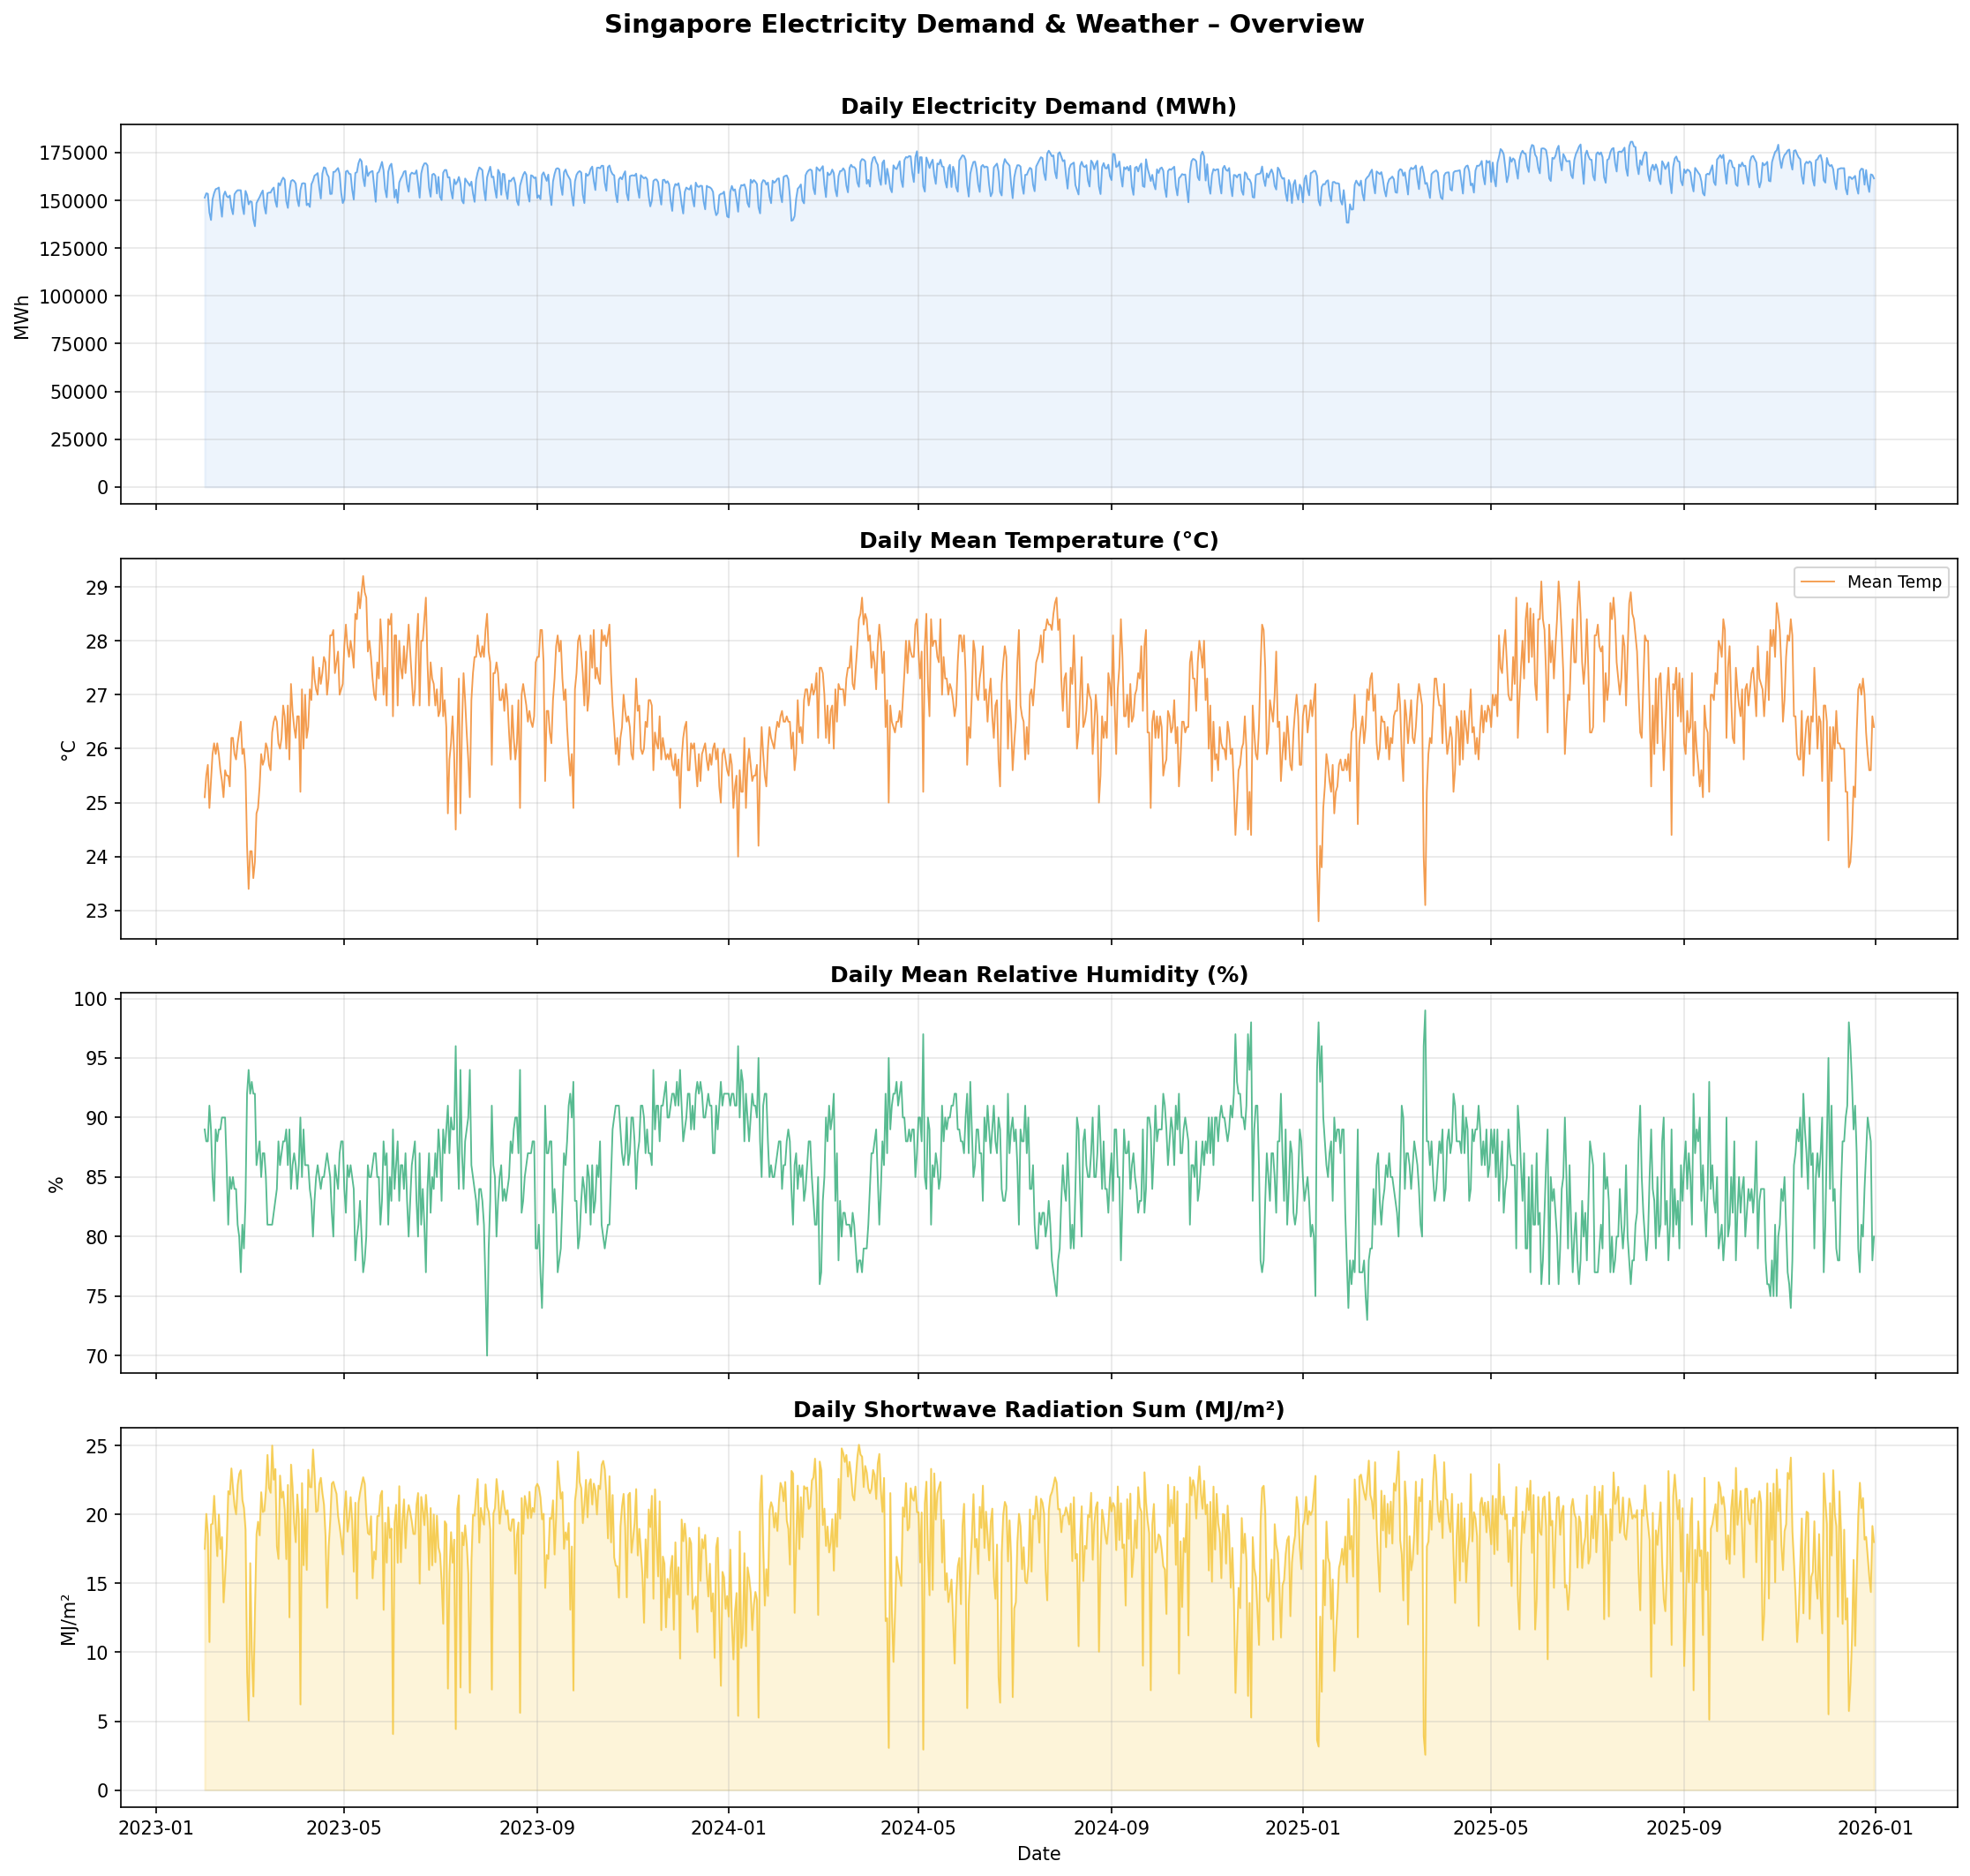
\includegraphics[width=0.95\textwidth]{background/images/eda_time_series.png}
    \caption{Daily electricity demand time series for Singapore (February 2023 -- December 2025), showing seasonal patterns and day-to-day variability.}
    \label{fig:demand_timeseries}
\end{figure}

Figure~\ref{fig:demand_timeseries} shows the daily electricity demand time series used in this study. The data exhibits clear weekly cyclicity (lower weekend demand), seasonal variation (higher demand during drier, hotter months), and occasional demand drops associated with public holidays.


\section{Conclusions}

This chapter has reviewed the theoretical foundations of electricity demand forecasting, from classical statistical methods to modern machine learning approaches. The CatBoost algorithm and its native handling of categorical features make it well-suited for the multi-type feature set used in this project. The PPSO meta-heuristic provides an efficient, parameter-free mechanism for optimising CatBoost's hyperparameters. The six evaluation metrics adopted from the reference study enable a rigorous and multi-dimensional comparison of model performance. The following chapter presents the system design that operationalises these methods into a cohesive forecasting pipeline.
